\chapter{Probability}

\begin{multicols}{2}[\subsubsection*{Contents of this chapter}]
   \printcontents{}{1}{\setcounter{tocdepth}{2}}
\end{multicols}


\section{Interpretations and Definitions of Probability}

\subsection{Naive and Non-Naive Definitions of Probability}
Probability courses typically start with what \citeasnoun{blitzstein2019introduction} calls the \textit{naive} definition of probability, which is to look at the fraction of the event space that corresponds to a particular event. This works well for combinatorial type of probability problems, such as the likely outcome of dice throws. The dichotomy below is from \citeasnoun{blitzstein2019introduction}.

\subsubsection{Naive Probability}
The event space $S$ consists of a collection of equally likely outcomes. The actual outcome $s_{actual} \in S$. The probability of an outcome in a subset $A\subseteq S$, $P(s_{actual}\in A)$ corresponds to the fraction of events in $A$ out of $S$.

\begin{equation}
P_{naive}(A) = \frac{|A|}{|S|} = \frac{\mathrm{number of outcomes favorable to A}}{\mathrm{total number of outcomes in S}}
\end{equation}

This approach runs into trouble when the outcomes in $|A|$ are not equally likely, or if the sample space is infinite, i.e. $|S|=\infty$.


\subsubsection{Non-Naive Definition of Probability}
A probability space consists of a sample space $S$ in addition to a \textit{probability function}. The job of the probability function is to take an event $A\subseteq S$ and map it to a number between $0$ and $1$. I.e.  $P: S \rightarrow [0,1]$.

The function $P$ must satisfy:

\begin{itemize}
\item P(\empty) = 0, P(S) = 1
\item If $A_1, A_2,...$ are \textit{disjoint} events, then: \begin{equation}P\left(\bigcup^{\infty}_{j=1}A_j \right) = \sum_{j=1}^{\infty}P(A_j)\end{equation}
\end{itemize}

In other words, all you need to work with probability is a set of possible outcomes $S$ and some function to apply to parts of that set.

\subsection{Frequentist Probability}
The \textit{frequentist} interpretation of probability is that it represents the frequency of an outcome of a particular experiment upon running the experiment many times. On one hand, this view on probability is arguably empirically grounded. On the other hand it relies on the impractical notion of identically repeating something a large number of times. 

\subsection{Bayesian Probability}
The \textit{Bayesian} view on probability is that it represents a degree of belief in a particular outcome. On one hand, this implies a degree of subjectivity. On the other hand, this notion of probability is much more broadly applicable, because it does not require repeatable experiments. It also permits the introduction of subjective biases through priors.

I'm not sure whether the supposed "battle" between frequentists and Bayesians has ever been of any consequence for me. Also, the frequentist perspective strikes me as inherently contradictory, because supposed empirical proof can strictly speaking never be practically delivered.

In practice, it seems that frequentist approaches tend to be structured around parametrization of solutions in terms of summary statistics, while Bayesians have a tendency to approach problems in terms of full probability distributions. Social scientists seem to be leaning towards frequentist methods, while physicists and engineers seem to be more interested in Bayesian data analysis. 

I suspect that an additional source of bias is that frequentist methods tend to be computationally lighter and that many standard accepted recipes exist for common problems. In contrast, Bayesian approaches are usually derived ad-hoc in the context of a particular problem.

\subsection{Measure Theoretic Probability}
The modern approach to probability is rooted in measure theory. In that context:

\begin{itemize}
\item The \textit{sample space} is a measurable set
\item An \textit{event} is a measurable set; a subset of the sample space.
\item A \textit{random variable} is a measurable function on the sample space.
\item The \textit{expectation} of a random variable is its integral with respect to the probability measure.
\end{itemize}


	




% mutually exclusive
\section{Mutually Exclusive Events, Disjoint Sets}
Two events $A$ and $B$ are mutually exclusive if $A\cap B= \emptyset$. That is, $A$ and $B$ are disjoint sets.

% independent 
\section{Independent Events}
Interestingly, independence can, with the exception of specific symmetric cases, generally not be read off from a Venn diagram \cite{wasserman2013all}. A set of events $A_i$ is \textit{independent} if:

\begin{equation}
\mathbb{P}\left(\bigcap_i A_i \right) = \prod_i \mathbb{P}(A_i)
\end{equation}

\citeasnoun{wasserman2013all} writes independence using the coproduct symbol $A\coprod B$. Independence can be either assumed or it can be proven by verifying $\mathbb{P}(A\cap B) = \mathbb{P}(A)\mathbb{P}(B)$.


% conditional probability
\section{Conditional Probability}
Conditional probability $\mathbb{P}(A|B)$ "probability of $A$ given $B$" is the ratio of the probability measure applied to the subsets $A\cap B$ and $B$:

For $\mathbb{P}(B) > 0$:
\begin{equation}
\mathbb{P}(A|B) = \frac{\mathbb{P}(A\cap B)}{\mathbb{P}(B)}
\end{equation}

For dependent events, this can be interpreted as the fraction of $B$ that overlaps with $A$. For independent events, $\mathbb{P}(A|B) = \mathbb{P}(A)$. 



% law of total expectation / tower rule
\section{Law of Total Probability}

Let $A_1,...,A_n$ be a partition of $\Sigma$ so that $\mathbb{P}(\bigcup_i A_i) = \mathbb{P}(\Omega) = 1$. Then:

\begin{equation}
\mathbb{P}(B) = \sum_i \mathbb{P}(B|A_i)\mathbb{P}(A_i) 
\end{equation} 

% Bayes Theorem
\section{Bayes' Theorem}
Let $A_1,...,A_n$ be a partition of $\Sigma$ so that $\mathbb{P}(\bigcup_i A_i) = \mathbb{P}(\Omega) = 1$ and $\mathbb{P}(A_i)>0$ for each $A_i$. Then:

\begin{equation}
\mathbb{P}(A_i|B) = \frac{\mathbb{P}(B|A_i)\mathbb{P}(A_i) }{\sum_j \mathbb{P}(B|A_j)\mathbb{P}(A_j) } = \frac{\mathbb{P}(B|A_i)\mathbb{P}(A_i) }{\mathbb{P}(B)}
\end{equation}

The theorem is so important that the different terms have names:

\begin{itemize}
\item $\mathbb{P}(A_i|B)$ is the posterior
\item $\mathbb{P}(B|A_i)$ is the likelihood 
\item $\mathbb{P}(A_j)$ is the prior
\item $\mathbb{P}(B)$ is the evidence
\end{itemize}

	




\section{Functions of Random Variables, Derived Distributions}

(This section needs revision)

I find changes of variables to be the easiest to understand by writing down a joint probability distribution using a delta function to express the conditional probability for the new variables based on the old variables. The next step is to perform a change of variables in the delta function, and integrate. The delta function means that the relationship between the old and the new variables is deterministic. If the relationship is non-deterministic you can use whatever expression for the conditional probability is appropriate.

Let's say that you want to know the probability distribution of the function $\vec{u} = \mathbf{H}(\vec{x})$ of some random variable $\vec{x}$ for which the probability distribution is known.

I personally find it least confusing to approach this problem by thinking about the joint probability distribution, and then obtaining $p(\vec{u})$ through marginalization:

\begin{equation}
p(\vec{u}) = \int dx^n p(\vec{x},\vec{u}) = \int dx^n p_x(\vec{x}) p_u(\vec{u}|\vec{x})
\end{equation}

Since $\vec{u}$ is a deterministic function of $\vec{x}$, the conditional probabiltiy $p_u(\vec{u}|\vec{x}) = \delta(\vec{u} - \mathbf{H}(\vec{x}))$. Explicitly:

\begin{equation}
p(\vec{u}) = \int dx^n p_x(\vec{x}) \delta(\vec{u} - \mathbf{H}(\vec{x}))
\end{equation}

What this does, is to integrate over all the points $p_x(\vec{x})$ where the argument of the delta function is zero. The important thing is that care needs to be taken when the argument of the delta function is itself a function. In that case, a change of variables has to be performed, so that this is no longer the case. On wikipedia, this is done by defining the new variable $du = |\frac{d}{dx}g(x)|dx$, from which follows:

\begin{equation}
\delta(g(x)) = \sum_{x_0} \frac{\delta(x-x_0)}{|g'(x_0)|}
\end{equation}

Where it is necessary to sum over each point $x_0$ for which $g(x_0) = 0$.

Which makes sense. Except, if you rewrite in terms of the new variable, you get an expression that does not strike me as necessarily the same:

\begin{equation}
\int f(x) \delta(g(x))dx = \sum_{n}\int f(g_n^{-1}(u)) \delta(u) \left|\frac{d}{du}g^{-1}(u)\right|du
\end{equation}

Where the sum $n$ is over all functions $g_n^{-1}$ that satisfy $g(g_n^{-1}(u)) = u$. For example, if $u = g(x) = sin(x)$ then $g_n^{-1} = asin(u) + n2\pi$, for any integer $n$. I feel more comfortable with the second path. The answer to my confusion is most likely the inverse function theorem (cf. section \ref{sec:inverse_function_theorem}). In other words: this section needs revision! But hey, I flagged it.

Note that a delta function with a vector argument can be written as a product of the delta functions along each dimension.

Define a new set of variables $\vec{a} = \vec{u} - \mathbf{H}(\vec{x})$. It follows that $\vec{x} = \mathbf{H_n^{-1}}(\vec{u}-\vec{a})$ and the volume element $dx^n = \left| \frac{d}{d\vec{a}}\mathbf{H}_n^{-1}(\vec{u}-\vec{a})\right|da^n$. Here, $H^{-1}_n$ are all the functions that satisfy $\mathbf{H}(\mathbf{H}_n^{-1}(\vec{u})) = \vec{u}$. The integral becomes:

\begin{equation}
p(\vec{u}) = \int da^n p_x(\mathbf{H}^{-1}_n(\vec{u}-\vec{a}))\left| \frac{d}{d\vec{a}}\mathbf{H}_n^{-1}(\vec{u}-\vec{a})\right| \delta(\vec{a})
\end{equation}

At this point it is safe to evaluate the delta function integral. The result is:

\begin{equation}
p(\vec{u}) = p_x(\mathbf{H}^{-1}_n(\vec{u})\left| \frac{d}{d\vec{a}}\mathbf{H}_n^{-1}(\vec{u}-\vec{a})\right|_{(\vec{a}=0)}
\end{equation}

\subsection{Example: Sum of Random Variables}
If the map $\mathbf{H}$ is not bijective, for example because $\vec{u}$ has lower dimensionality than $\vec{x}$, then a bijective map can be artifically constructed by introducing additional variables that are then also marginalized out. For example, if the goal is to calculate the probability of measuring some sum of random variables $s$, then you can define:

\begin{equation}
u_0 = s - \sum(x_i)\\
u_1 = x_1\\
u_2 = x_2\\
\vdots\\
u_{(n-1)} = x_{n-1}
\end{equation}

The inverse is:

\begin{equation}
x_1 = u_1\\
x_2 = u_2\\
\vdots\\
x_n = s - u_0 - \sum_{i<n} x_i
\end{equation}

The argument in the delta function is transformed $\delta(s - \sum(x_i)) \rightarrow \delta(u_0)$. The determinant of the Jacobian $|J| = |\frac{d}{d\vec{u}} H^{-1}(\vec{u})|$ is given by $[\frac{d}{du_1} \mathbf{H^{-1}},\frac{d}{du_2} \mathbf{H^{-1}},...,\frac{d}{du_{n-1}} \mathbf{H^{-1}}]$. That's an $nxn$ matrix where the first row is all $-1$, the lower left is an $(n-1)x(n-1)$ identity matrix, and the lower right is a $(n-1)x1$ vector of 0s. The determinant is one. Consequently the probability distribution of measuring a sum $s$ is given by:

\begin{equation}
p(s)= \int dx^{n-1} p_x(x_1,x_2,x_3,...,s-\sum_{x<n}x_i)
\end{equation}

Which turns out to be the convolution when the variables are independent.

\subsection{Example: Lower Dimensional Random Variable}

This was already the case for the sum of several random variables, in which case the dimensionality of the problem was reduced from many to one. 

Consider the case many to fewer. Again, you just need to perform a change of variables. The new set of variables needs to have the same dimensionality as the old set of variables. The rest should follow pretty obviously. 

Linear example: $\vec{y} = \mathbf{M}\vec{x}$ where $y$ has 2 dimensions and $x$ has 3. 

Transform:

\begin{equation}
u_1 = y_1 - \vec{M_1}\cdot\vec{x}\\
u_2 = y_2 - \vec{M_2}\cdot\vec{x}\\
u_3 = x_3
\end{equation}

You can write this in terms of some invertible matrix $\mathbf{W} = [\mathbf{M},[0,0,1]]$ as $\vec{u} = \mathbf{W}\vec{x}$, so that $dx^n = |\mathbf{W}^{-1}|du^n|$. The integral is then:

\begin{equation}
p(y) = \int du^n p_x(\mathbf{W}^{-1}(\vec{y}-\vec{u}))\delta(u_1)\delta(u_2)|\mathbf{W}^{-1}|
\end{equation}

\section{Indicator Variables}

Indicator variables are useful devices that simplify probability calculations involving binary outcomes, namely wether the outcome lies in a certain region of event space or not. Specifically, they allow one to translate set expressions into algebraic expressions. 

Let $A\subseteq S$ be a subset of event space $S$ (ex. $A\equiv$ "it rains tomorrow"). Then the indicator variable $I_A$: 

\begin{equation}
I_A = \left\{\begin{array}{l} 1 \mathrm{\ if\ outcome\ in\ A}\\0 \mathrm{\ if\ outcome\ in\ A^c} \end{array}\right.
\end{equation}

Which means that:
\begin{equation}
\mathbb{E}(I_A) = 1\times p(A) + 0\times p(A^c)= p(A)
\end{equation}

To indicator variables for different events $A,B,C...$ can also be combined:
\begin{equation}
I_{A\cap B\cap C\cap ...} = I_A I_B I_C ...
\end{equation}

And indicator variables for the complement can be constructed trivially:
\begin{equation}
I_{A^c} = 1 - I_A
\end{equation}

Whenever accounting for complicated combinations of events becomes overwhelming, indicator variables are often a good approach.

\subsection{Example: The Party Problem}

The party problem is a typical interview question, so I will include the two easier problems that do not make use of indicator variables. (This version of my notes also still has bitterness included.)

There are $n$ drunk kids at a party that is presumably getting shut down by the fun police in Cambridge, MA. They (meaning the kids, presumably) grab their coats at random, and the problem is built around thinking about how many people wind up with the correct coat.

\subsubsection{Lame Interview Question 1: Every one finds their coat}
The common version of this problem asks "what is the probability that all of the kids wind up with the right coat". This is much easier than the general case. Imagine the list of party guests as a sequence $(1,2,3,4,...,n-1,n)$ and the coats they grab as a random permutation of that sequence, such as $\alpha = (6,1,40,21,9,...)_n$. There are $n!$ such permutations, and they are all equally likely. The probability of all guests getting the correct coat is the probability that the permutation happens to be the single correct one, i.e. $p(\alpha = (1,2,3,4,...,n-1,n)_n)$, which is the probality of one particular permutation, i.e. $p(\alpha = (1,2,3,4,...,n-1,n)_n) = \frac{1}{n!}$.

\subsubsection{Lame Interview Question 2: At least r people find their coat}
This is still pretty easy, because the permutations that are correct are easily counted. If at least $r$ coats are correctly assigned, then there are $\left(\begin{array}{l}n\\r\end{array}\right)$ ways of choosing wich of the $r$ people wind up with the right coat. Then, while the location of $r$ indices in the sequence is fixed, $n-r$ indices can be assigned arbitrarily.

The number of permutations where at least $r$ are assigned correctly are then:

\begin{equation}
\left(
\begin{array}{l}
n\\
r
\end{array}
\right)(n-r)!
\end{equation}

And the probability of at least $r$ people finding their coat is the number of permutations multiplied with the probability of an individual permutation (that is, $\frac{1}{n!}$):

\begin{equation}
p(\mathrm{\#\ correct} \geq r)=\left(
\begin{array}{l}
n\\
r
\end{array}
\right)\frac{(n-r)!}{n!} = \frac{1}{r!}
\end{equation}

Where $r\leq n$.

\subsubsection{Not lame: Exactly r people find their coat}
So, then, what's the probability that exactly nobody finds their coat? What's the probability that 2 people find their coat but nobody else does? What's the probability that $r$ out of $n$ people find their coat? After thinking quickly on your feet for two seconds, you realize that the answer is obviously:

\begin{equation}
p(\mathrm{\#\ correct} = r) = \frac{1}{r!}\sum_{s=0}^{n-r} \frac{(-1)^s}{s!}
\end{equation}

The interviewer grunts ambiguously. They never call you back. You never find out why. You can't sleep. You can't eat. You become an anarchist and you declare war on the system.

The first two versions here are what I've come across in interview prep-type materials. I find them a bit annoying, because they represent particular cases that are much simpler than the general case. Applicants in the habit of studying stupid interview questions are rewarded because those answers are easily memorized (false positive). Applicants who intuit the complexity of the general problem, and who don't know the answer beforehand, might become overwhelmed during an interview and fail (false-ish negative).

/ rant

My approach here follows the extraordinary lecture notes https://mast.queensu.ca/~stat455/ by Glen Takahara at the University of Queensland. The difficulty of the problem is that events of a coat being picked up are interrelated: whether one person picks up their correct coat alters the probability of another person also picking up their correct coat. The beauty of this solution is that, rather than messing about with conditional probabilities, it looks at subsets of the event space, and then uses indicator variables to translate set expressions into algebraic expressions.

It uses the properties:

\begin{equation}
I_A = \left\{\begin{array}{l} 1 \mathrm{\ if\ outcome\ in\ A}\\0 \mathrm{\ if\ outcome\ in\ A^c} \end{array}\right.
\end{equation}

Which means that:
\begin{equation}
\mathbb{E}(I_A) = 1\times p(A) + 0\times p(A^c)= p(A)
\end{equation}

To indicator variables for different events can also be combined:
\begin{equation}
I_{A\cap B\cap C\cap ...} = I_A I_B I_C ...
\end{equation}

And indicator variables for the complement can be constructed trivially:
\begin{equation}
I_{A^c} = 1 - I_A
\end{equation}

Let $A_i$ be the region of state space in which guest $i$ grabbed the right coat. Let's say a *particular* subset $\{i\}_r$ of $r$ guests grabs their correct coats (for example, $\{i\}_r = \{5,9,11,24,...\}_r)$, and that the set of remaining $n-r$ guests $\{j\}_{n-r}= \{1,2,3,...\}_n\setminus\{i\}_r$ grab the wrong coat. The area of state space that corresponds to this outcome is:

\begin{equation}
A_{\{i\}_r,\{j\}_{n-r}}=\bigcap_{i\in\{i\}_r}A_i\bigcap_{j\in\{j\}_{n-r}}A_j^c
\end{equation}

The event that the outcome lies within that region of configuration space can be described with an indicator function:

\begin{equation}
I_{A_{\{i\}_r,\{j\}_{n-r}}} = \prod_{\{i\}_r}I_{A_i}\prod_{\{j\}_{n-r}}(1-I_{A_j})
\end{equation}

And the probability of those *particular* $r$ people finding their coat is it's expectation value, $p(A_{\{i\}_r,\{j\}_{n-r}}) = \mathbb{E}(I_{A_{\{i\}_r,\{j\}_{n-r}}})$. Good stuff.

The expression above will consist of a bunch of products of indicator variables that describe whether a particular guest wound up with the correct coat. We know that the product of indicator variables corresponds to an indicator variable for the *intersection* of the corresponding subsets of the state space. Explicitly, if it is a product of $s$ indicator variables for some particular set of coats coat $\{k\}_s$:

\begin{equation}
\prod_{k} I_{A_k} = I_{\bigcap_{k}A_k}
\end{equation}

And $\mathbb{E}(I_{\bigcap_{k} A_k}) = p(\bigcap_{k} A_k)$ is the probability of a particular $s$ coats being picked up correctly, which is $(n-s)!/n!$. (There is no binomial factor, because it's one *specific* set of $s$ coats).

Products of the sort $\prod^n (1-x_i)$ can be expanded:

\begin{equation}
\prod^n (1-x_i) = \sum_{s=0}^n (-1)^s \sum_{1\leq i_1,...,i_s\leq n} x_{i_1}x_{i_2}...x_{i_s}
\end{equation}

The sum $\sum_{1\leq i_1,...,i_s\leq n}$ is over all possible sets of up to $s$ indices that can be drawn from $\{1,2,3,...,n\}$. A simple example with $n=3$:

\begin{equation}
(1-x_1)(1-x_2)(1-x_3) = \underbrace{1}_{s=0} - \underbrace{(x_1 + x_2 + x_3)}_{s=1} + \underbrace{(x_1x_2 + x_2x_3 + x_1x_3)}_{s=2} - \underbrace{(x_1x_2x_3)}_{s=3}
\end{equation}

The number of terms of order $s$ is the amount of ways that $s$ indices can be sampled from $n$ indices, $\left(\begin{array}{l}n\\s\end{array}\right)$.

Returning to the original problem, then:

\begin{equation}
\begin{array}{ll}
I_{A_{\{i\}_r,\{j\}_{n-r}}} &= \prod_{\{i\}_r}I_{A_i}\prod_{\{j\}_{n-r}}(1-I_{A_j})\\
&=\sum_{s=0}^{n-r} (-1)^s \underbrace{\sum_{n-r\leq j_1,...,j_s\leq n}}_{\mathrm{sum\ of\ }\left(\begin{array}{l}n-r\\s\end{array}\right)\mathrm{\ terms\ \ }} \underbrace{\prod_{\{i\}_r} I_{A_i}\prod_{\{j\}_s}I_{A_j}}_{\mathrm{product\ of\ r+s\ terms\ \ }}
\end{array}
\end{equation}

By linearity of expected value, and using the relationship of the expected value of indicator variables to their probabilities:

\begin{equation}
\begin{array}{rl}
\mathbb{E}(I_{A_{\{i\}_r,\{j\}_{n-r}}}) &= \sum_{s=0}^{n-r} (-1)^s \underbrace{\sum_{n-r\leq j_1,...,j_s\leq n}}_{\mathrm{sum\ of\ }\left(\begin{array}{l}n-r\\s\end{array}\right)\mathrm{\ terms\ \ }} p\left(\underbrace{I_{\bigcap_{\{i\}_r}A_i\bigcap_{\{j\}_s}A_j}}_{\mathrm{r+s\ coats\ picked\ up\ correctly}}\right)\\
&=\sum_{s=0}^{n-r} (-1)^s \left(\begin{array}{c}n-r\\s\end{array}\right)\frac{(n-r-s)!}{n!}
\end{array}
\end{equation}

Now, this is already a pretty neat expression for the probability of a *particular* $r$ coats being picked up correctly (i.e. Joe, Mary, and "Hans" picked up the right coat). We don't really care which of the $r$ guests got lucky, though, so since there are $\left(\begin{array}{c}n\\r\end{array}\right)$ ways of $r$ coats having been picked out correctly, you sum over all of them:

\begin{equation}
\begin{array}{ll}
p(\mathrm{\#\ correct} = r) &= \left(\begin{array}{c}n\\r\end{array}\right) \sum_{s=0}^{n-r} (-1)^s \left(\begin{array}{c}n-r\\s\end{array}\right)\frac{(n-r-s)!}{n!}\\
&= \sum_{s=0}^{n-r} (-1)^s \frac{n!}{r!(n-r)!}\frac{(n-r)!}{s!(n-r-s)!}\frac{(n-r-s)!}{n!}\\
&= \frac{1}{r!}\sum_{s=0}^{n-r} \frac{(-1)^s}{s!}
\end{array}
\end{equation}


\begin{figure}
\centering
    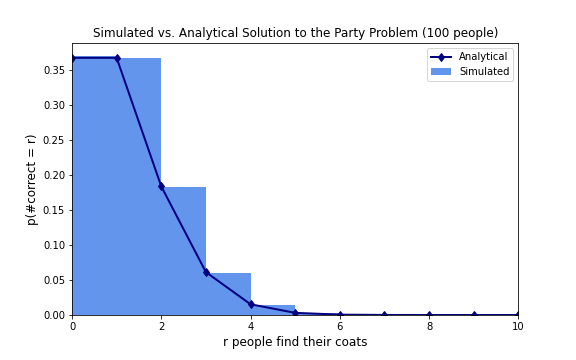
\includegraphics[width=0.7\textwidth]{partyproblem.png}
    \caption{Simulated and analytically calculated probabilities that exactly $r$ people at a $n=100$ people party randomly pick up their coat.}
    \label{fig:proba_partyproblem}
\end{figure}



\section{Copulas}


\section{Relationships Between Distributions}

\section{Large Deviation Theory}
\subsection{Gaertner-Ellis Theorem}
\subsection{Example: Sum of Uniform Random Variables}

\section{Point Mass Distributions}

If the entire probability is concentrated at a single point $\alpha$, then that can be expressed in terms of the Kronecker Delta in the discrete case and the Dirac Delta function in the continuous case.

\subsection{Kronecker Delta $\delta_{\alpha}$}
In the discrete case:

\begin{equation}
\delta_{\alpha} = \left\{\begin{array}{l} 1\mathrm{\ if\ }x = \alpha \\ 0\mathrm{\ else}\end{array} \right.
\end{equation}

\subsection{Dirac Delta Function $\delta(x-\alpha)$}
In the continuous case:

\begin{equation}
\int_A \delta(x-\alpha) \mathrm{d}x = \left\{\begin{array}{l} 1\mathrm{\ if\ }\alpha \in A \\ 0\mathrm{\ else}\end{array} \right.
\end{equation}

The Dirac Delta function is actually a distribution with extremely useful properties that I ought to write up. 

\section{Uniform Distributions}

\subsection{Discrete Uniform $\mathrm{Uniform(1,k)}$}
With $k>0$ be some integer, the PMF is:

\begin{equation}
f(x) = \left\{\begin{array}{l} 1/k \mathrm{\ if\ }x \in \{1,...,k\} \\ 0\mathrm{\ else}\end{array} \right.
\end{equation}

The CDF is:

\begin{equation}
F(x)= \left\{\begin{array}{cl} 
0& x < 1\\
\frac{x}{k}& 1\leq x \leq k\\
1& x>k
\end{array} \right.
\end{equation}

% continuous uniform
\subsection{Continuous Uniform $\mathrm{Uniform(a,b)}$}

With $a,b\in\mathbb{R}$ and $b>a$, the PDF is:

\begin{equation}
f(x) = \left\{\begin{array}{l} 1/(b-a) \mathrm{\ if\ }x \in [a,b] \\ 0\mathrm{\ else}\end{array} \right.
\end{equation}

The CDF is:

\begin{equation}
F(x)= \left\{\begin{array}{cl} 
0& x < a\\
\frac{x-a}{b-a}& a\leq x \leq b\\
1& x>b
\end{array} \right.
\end{equation}


% bernoulli 
\section{Bernoulli Processes}
A Bernoulli process is a number of discrete trials with binary outcome, for example a series of coinflips. This is typically framed in terms of success $X=1$ with probability $p$ and failure $X=0$ with probability $1-p$. The trials are independent from each other. Thinking of the process as a sequence in time, this means that the process is memoryless: the number of successes or time since the last success have no bearing on the future. Thinking about the process as a sequence in space, the successes are independently scattered over a grid like randomly flipped bits in a string of bits. That is, the events are uniformly distributed.


\subsection{Bernoulli $\mathrm{Bernoulli(p)}$}
The PMF of a single binary outcome $X=1$ with probability $p$ and $X=0$ with probability $1-p$. The PMF is:

\begin{equation}
f(x) = p^x (1-p)^{1-x} =  \left\{\begin{array}{cl} 
p& x = 1\\
(1-p)& x=0
\end{array} \right.
\end{equation}

For $x\in\{0,1\}$ and $p\in[0,1]$.


% binomial
\subsection{Binomial $\mathrm{Binomial}(n,p)$}
The binomial distribution is the PMF for the number of successes with probability $p$ among $n$ trials. That is, if $X_i \sim \mathrm{Bernoulli}(p)$, then $X = \sum_i^n X_i$ has distribution:

\begin{equation}
f(x) = {n \choose x} p^x (1-p)^{n-x}
\end{equation}

It follows that if $X_1 \sim \mathrm{Binomial}(n_1,p)$ and $X_2 \sim \mathrm{Binomial}(n_2,p)$, then $X_1 + X_2 \sim \mathrm{Binomial}(n_1+n_2,p)$. The binomial distribution can be interpreted of the probability that there will be $x$ successes among $n$ draws with replacement.


% geometric distribution
\subsection{Geometric $\mathrm{Geom}(p)$}
The PMF for the number of Bernoulli trials with parameter $p\in(0,1)$ is given by: 

\begin{equation}
f(x) = p(1-p)^{x-1}
\end{equation}

In the time picture, it models the number of intervals $x$ until the first success occurs, or, equivalently, the number of trials between two successes. In the space picture, it models the distance between successes that are independently scattered on a grid.



% negative binomial distribution
\subsection{Pascal, Negative Binomial $\mathrm{NB}(r,p)$}
The negative binomial distribution with parameters $r$ and $p$ gives the sum of $r$ geometric random variables with parameter $p$. In the time picture, if $X \sim \mathrm{NB}(r,p)$, $X$ gives the probability for the number of failures in a sequence of Bernoulli trials until there are $r$ successes. In the space picture, it the probability for the width of the interval of a grid between $r$ successes (not counting the spots taken up by the successes). Its PMF is given by:

\begin{equation}
f(x) = {x+r-1\choose x} p^r (1-p)^x
\end{equation} 

For $r=1$, the distribution is the same as the geometric distribution with parameter $p\rightarrow 1-p$. The negative binomial distribution gives the probability that, when drawing with replacement, it will take $x$ failures until there have been $r$ successes, where each success has probability $p$.

% bernoulli without replacement
\section{Bernoulli Processes 	Without Replacement}
Bernoulli Processes were a sequence of independent trials, which can be thought of as a sequence of samples with replacement. The "hyper"- distributions treat the analogous case where samples are not replacemed.  

% hypergeometric distribution
\subsection{Hypergeometric $\mathrm{Hypergeom(N,K,n)}$}
The hypergeometric distribution gives the probability for the number of successes when drawing $n$ times from a population of $N$, of which $K$ correspond to successes.

\begin{equation}
f(k) = \frac{{K \choose k}{ N-K \choose n-k}}{{N \choose k}}
\end{equation} 

It is the analogue to the binomial distribution for sampling without replacement.

% negative hypergeometric distribution
\subsection{Negative Hypergeometric $\mathrm{NH(N,K,n)}$}
The negative hypergeometric distribution gives the probability that, when sampling without replacement, it will take $r$ failures until there have been $k$ successes, if the total population is $N$ and the number of elements corresponding to a success is $K$.

\begin{equation}
f(k) = \frac{{k+r-1\choose k}{N-r-k \choose K-k}}{{N\choose K}}
\end{equation}

The negative hypergeometric distribution is the analogue to the negative binomial distribution for sampling without replacement. 


% poisson processes
\section{Poisson Point Processes}
Poisson point processes are the continuous analogue to Bernoulli processes. Rather than looking at the outcome of a number of binary trials, they look at the number or spacing of independent point events over a continuous interval. In one dimension, Poisson Processes very often model rare events happening over a given time interval. In higher dimensions, the Poisson process can be thought of as independently scattered points in some volume. The process is typically characterized by the parameter $\Lambda$, called the \textit{rate} or \textit{intensity} of the process. It can be written $\Lambda = \nu \lambda$ where $\nu$ is a Lebesgue measure (assigning a length or volume to a set) and $\lambda$ is a constant. For a temporal process, $\nu$ would be the time interval. For a spatial process, $\nu$ would be a volume. The events have uniform distribution over the measure. This is also called a homogenous Poisson process. 

% poisson distribution
\subsection{Poisson $\mathrm{Poisson}(\Lambda)$}
The poisson distribution is the continuous analogue to the Binomial distribution. It measures the number of events for a process with intensity $\Lambda$.

\begin{equation}
f(x) = e^{-\Lambda}\frac{\Lambda^x}{x!}\ \ \mathrm{x\geq0}
\end{equation}

Just like for the Binomial distribution, if $X_1 \sim \mathrm{Poisson}(\Lambda_1)$ and $X_2 \sim \mathrm{Poisson}(\Lambda_2)$, then $X_1 + X_2 \sim \mathrm{Poisson}(\Lambda_1 + \Lambda_2)$. 

The mean and variance of the poisson distribution are both $\lambda$. This link means that Poisson distributed data is inherently heteroskedastic. The Poisson distribution can be obtained from the Bernoulli distribution by considering a very large number of trials with a small probability of success in each trial. That is, if $Y \sim B(n,\pi)$ then letting $n\rightarrow \infty$ with $\pi \rightarrow 0$ and $\mu \rightarrow n\pi$ you recover the Poisson distribution. In this sense, the Poisson distribution is an approximation to a Binomial process with rare events with large $n$ and small $\pi$. 



% exponential distribution
\subsection{Exponential $\mathrm{Exp}(\lambda)$}
The exponential distribution is the continuous analogue to the Geometric distribution. In one dimension, if $X \sim \mathrm{Exp}(\Lambda)$, then $X$ can be interpreted as the distance between two independently scattered points on the real line. In the time picture, that would be the time that elapses between two events, or, equivalently, the time until the next event, where $\lambda$ is the rate or intensity.

\begin{equation}
f(x) = \lambda e^{-\lambda}
\end{equation}


% gamma distribution
\subsection{Gamma $\mathrm{Gamma(\alpha,\beta)}$}
The Gamma Distribution is the continuous analogue to the negative binomial distribution. For integer $\alpha$, it gives the probability of the value of the sum of $\alpha$ exponentially distributed random variables with parameter $\beta=\frac{1}{\lambda}$. That is, if $X_i \sim Exp(\frac{1}{\beta})$ then $X = \sum_i^\alpha X_i \sim \mathrm{Gamma}(\alpha,\beta)$. The PDF is given by:

\begin{equation}
f_x = \frac{1}{\beta^\alpha \Gamma(\alpha)}x^{\alpha-1}e^{-x/\beta}
\end{equation}

With $\alpha,\beta > 0$.

As one would expect, if $X_1 \sim \Gamma(\alpha_1,\beta)$ and $X_2 \sim \Gamma(\alpha_2,\beta)$ then $X_1 + X_2 \sim \Gamma(\alpha_1+\alpha_2,\beta)$. 



% t distribution
\section{$t$-Distribution $\mathrm{t_\nu\ }$}

\subsection{Cauchy Distribution $t_1$}
The Cauchy Distribution does not have a mean. It is infinite.


\section{Chi$^2$-Distribution $\chi^2_p$}
The $\chi^2$ distribution is the probability distribution of the sum of squares of standard normally distributed random variables. If $Z_i$ has standard normal distribution, then $X = \sum_i^p Z_i \sim \chi^2_p$.


% normal
\section{Normal $\mathscr{N}(\mu,\sigma^2)$}


\subsection{Standard Normal Distribution $\mathscr{N}(0,1)$ }

The normal distribution is so ubiquitous that there is notation specifically for the \textit{standard normal distribution}, which is the normal distribution with parameters $\mu = 0$ and $\sigma = 1$. It is always possible to transform a random variable $X$ to have standard normal distribution by performing a coordinate transform. The PDF of the standard normal distribution is written $\phi(x)$ and the CDF $\Phi(x)$. The PDF is given by: 

\begin{equation}
\phi(x) = \frac{1}{\sqrt{2\pi}}\exp{-x^2}
\end{equation}

The CDF has no closed form expression. 

By convention, $Z$ is the random variable that has standard normal distribution. If $X \sim \mathscr{N}(\mu,\sigma^2)$, then $Z = \frac{X-\mu}{\sigma} \sim \mathscr{N}(0,1)$. This standardizing transformation allows for calculations using lookup tables. 

\subsubsection{Example: Interval $\mathbb{P}(a<X<b)$}

\begin{equation}
\mathbb{P}(a<X<b) =  \mathbb{P}(a' < Z < b') = \Phi(b') - \Phi(a')
\end{equation}

with $a' = \frac{a-\mu}{\sigma}$ and $b' = \frac{b-\mu}{\sigma}$.

\subsubsection{Example: Quantile $x = F^{-1}(q)$}

\begin{equation}
z = \Phi^{-1}(q)
\end{equation}

with $z = \frac{x-\mu}{\sigma}$, so that $x = \sigma \Phi^{-1}(q)+\mu$. The interquartile range is calculated by transforming $(z_{1}=\Phi^{-1}(0.25),z_{3}=\Phi^{-1}(0.75))$, and so on.


% log normal 
\section{Log Normal Distribution}
The log normal distribution has the odd property that is ``thin tailed" for low variance and ``fat tailed" for high variance.

% Multinoulli Processes
\section{Categorial Processes, Multinoulli Processes}
A Multnoulli process is a number of discrete trials that may assume a number of different categorical outcomes, for example a series of dice throws or a random sequence of letters. It is the generalization of the Bernoulli process to processes with more than two possible outcomes. The trials are independent from each other. Thinking of the process as a sequence in time, this means that the process is memoryless: the sequence of future outcomes is independent of past outcomes. Thinking about the process as a sequence in space, it is a uniformly random assignment of one of a set number of outcomes to grid points.

% Multinoulli
\subsection{Categorical, Multinoulli $\mathrm{Categorical(\mathbf{p})}$}
The categorial or Multinoulli distribution is the generalization of the Bernoulli distribution to more than two possible outcomes. The PMF is given by:

\begin{equation}
f(\mathbf{x}) = \prod_i^k p_i^{[x=k]}
\end{equation}

With $p_i \in \mathbf{p}$ a discrete probability distribution and $[x=k]$ is the Iverson bracket.

% Multinomial
\subsection{Multinomial $\mathrm{Multinomial(n,\mathbf{p})}$}
The multinomial distribution is the multivariate generalization of the binomial process. Rather than a binary outcome, there are $k$ possible outcomes. If $\mathbf{X}=(X_1,X_2,...,X_k)$ has multinomial distribution with parameter vector $\mathbf{p} = (p_1,p_2,...,p_k)$, then it gives the probability that out of $n$ trials, $x_j$ will be of type $j$, where the probabilities of the different classes is given by the discrete probability distribution $\mathbf{p}$.

\begin{equation}
f(\mathbf{x}) = {n \choose x_1,x_2,...,x_k} p_1^{x_1}p_2^{x_2}...p_k^{x_k} = {|\mathbf{x}|\choose \mathbf{x}}\mathbf{p}^{\mathbf{x}}
\end{equation}

Where the final expression uses multi-index notation. The binomial process corresponds to $k=2$ classes (success and failure). The marginal distribution of $X_j$ is $Binomial(n,p_j)$.


% beta distribution
\section{Beta $\mathrm{Beta}(\alpha,\beta)$}

The PDF for the beta distribution is:

\begin{equation}
f(x) = \frac{\Gamma(\alpha + \beta)}{\Gamma(\alpha)\Gamma(\beta)}x^{\alpha-1}(1-x)^{\beta-1}\ \ 0 < x < 1
\end{equation}

With $\alpha, \beta > 0$.

The Beta distribution is the conjugate prior to the Bernoulli and Binomial distributions.

% dirichlet distribution
\section{Dirichlet $\mathrm{Dirichlet}(\mathbf{\alpha})$}
The Dirichlet Distribution is the multivariate generalization of the Beta Distribution. Given $\mathbf{X} = (X_1,...,X_K)$ and the parameter vector $\mathbf{\alpha} = (\alpha_1,...,\alpha_K),\ \alpha_j > 0$, the PDF is:

\begin{equation}
f(\mathbf{x},\mathbf{\alpha}) = \frac{1}{B(\mathbf{\alpha})} \prod^K_{i=1} x_i^{\alpha_i -1}
\end{equation}

Where $B(\mathbf{\alpha})$ is the multivariate Beta function:

\begin{equation}
B(\mathbf{\alpha}) = \frac{\prod^K_{i=1}\Gamma(\alpha_i)}{\Gamma(\sum_{i=1}^K\alpha_i)}
\end{equation}

The Dirichlet distribution is the conjugate prior to the Multinoulli/Categorical and Multinomial distributions. The marginal distributions are Beta distributions, i.e. $X_i \sim \mathbf{Beta}(\alpha_i,\alpha_0-\alpha_1)$ where $\alpha_0 = \sum_j \alpha_j$.



% multivariate normal distribution
\section{Multivariate Normal $\mathscr{N}(\mathbf{\mu},\mathbf{\Sigma})$}
The multivariate normal distribution is the multivariate generalization of the normal distribution. The PDF is given by:

\begin{equation}
f{\mathbf{x}} = \frac{1}{(2\pi)^{\frac{k}{2}}|\Sigma|^{\frac{1}{2}}}\exp\{-\frac{1}{2}(\mathbf{x}-\mathbf{\mu})^T \mathbf{\Sigma}^{-1}(\mathbf{x}-\mathbf{\mu})\}
\end{equation}



% covariance matrix
\subsection{Covariance Matrix $\mathbf{\Sigma}$}
The covariance matrix $\mathbf{\Sigma}$ is symmetric and positive definite. Therefore, $\mathbf{\Sigma}^{\frac{1}{2}}$ exists and is real, symmetric, and

\begin{itemize}
\item $\mathbf{\Sigma}^{\frac{1}{2}}\mathbf{\Sigma}^{\frac{1}{2}} = \mathbf{\Sigma}$
\item $\mathbf{\Sigma}^{\frac{1}{2}}\mathbf{\Sigma}^{-\frac{1}{2}}=\mathbf{\Sigma}^{-\frac{1}{2}}\mathbf{\Sigma}^{\frac{1}{2}}=\mathbf{I}$
\end{itemize}


% marginal distribution 
\subsection{Marginal Distribution}
If $\mathbf{X} \sim \mathscr{N}(\mathbf{0},\mathbf{\Sigma})$, then the marginal distribution of $X_a$ is:

\begin{equation}
X_a \sim \mathscr{\mu_a,\Sigma_{aa}}
\end{equation}


% conditional distribution
\subsection{Conditional Distribution}
If $\mathbf{X} \sim \mathscr{N}(\mathbf{0},\mathbf{\Sigma})$, then the conditional distribution of $X_b$ given $X_a = x_a$ is:

\begin{equation}
X_b|X_a = x_a \sim \mathscr{N}(\mu_b + \Sigma_{ba}\Sigma_{aa}^{-1}(x_a - \mu_a), \Sigma_{bb}-\Sigma_{ba}\Sigma_{aa}^{-1}\Sigma_{ab}) 
\end{equation}


% vector multiplication 
\subsection{Vector Multiplication}
If $\mathbf{a}$ is a vector, then:

\begin{equation}
\mathbf{a}^T \mathbf{X} \sim \mathscr{N}(\mathbf{a}^T \mathbf{\mu}, \mathbf{a}^T\mathbf{\Sigma}\mathbf{a})
\end{equation}


% relationship to chi2
\subsection{Relationship to Chi$^2$}
\begin{equation}
V = \mathbf{Z}^T\mathbf{Z} = (\mathbf{X}-\mathbf{\mu})^T\mathbf{\Sigma}^{-1}(\mathbf{X}-\mathbf{\mu}) \sim \chi^2_k
\end{equation}

\subsection{Multivariate Standard Normal Distribution $\mathscr{N}(\mathbf{0},\mathbf{\Sigma})$}
The standard multivariate normal distribution for $\mathbf{Z} = (Z_1,...,Z_k)$ with $\mathbf{Z} \sim \mathscr{N}(\mathbf{0},\mathbf{I})$ is:

\begin{equation}
f(z) = \prod^k_{i=1} f(z_i) = \frac{1}{(2\pi)^{\frac{k}{2}}}\exp \{ \frac{1}{2} \sum^{k}_{j=1} z_j\} = \frac{1}{(2\pi)^{\frac{k}{2}}}\exp \{ \frac{1}{2} \mathbf{z^T z}\}
\end{equation}

The transformation to a general multivariate normal random variable $\mathbf{X}$ is that if $\mathbf{Z} \sim \mathscr{0,\mathbf{I}}$, then $\mathbf{X} = \mathbf{\mu} + \mathbf{\Sigma}^{\frac{1}{2}}\mathbf{Z}$. Conversely, if $\mathbf{X}\sim \mathscr{\mathbf{\mu},\mathbf{\Sigma}}$ then $\mathbf{\Sigma}^{-\frac{1}{2}}(\mathbf{X}-\mathbf{\mu}) \sim \mathscr{N}(0,\mathbf{I})$.
	

% Expectations
\section{Expectations}

\subsection{Law of the Unconscious Statistician}
Given a random variable $X$ with distribution $f(x)$ and some function $r(x)$, the expected value $\mathbb{E}(r)$ is given by:

\begin{equation}
\mathbb{E}(r) = \int r(x) \mathrm{d}F_X(x)
\end{equation}

\subsection{Linearity of Expeced Value}
\begin{equation}
\mathbb{E}\left(\sum_i a_i X_i \right) = \sum_i a_i \mathbb{E}(X_i)
\end{equation}

% Moments
\section{Moments, Central Moments}

The $k$th moment is $\mathbb{E}X^k$. The $k$th central moment is $\mathbb{E}(X-\mu)^k$.


% Variance
\section{Variance}

In one dimension:
\begin{equation}
\sigma^2 =\mathbb{V}(X) = \mathbb{E}(X-\mu)^2 = \int (x-\mu)^2 \mathrm{d}F(x)
\end{equation}

The standard deviation is $\mathrm{sd}(X) = \sqrt{\mathbb{V}(X)}$. 

\begin{itemize}
\item $\mathbb{V}(X) = \mathbb{E}(X^2) - \mu^2$.
\item If $a$ and $b$ are constants, $\mathbb{V}(aX+b) = a^2 \mathbb{V}(X)$.
\item If $X_1,...,X_n$ are independent and $a_1,...,a_n$ are constants, then $\mathbb{V}\left(\sum^n_{i=1}a_i X_i\right) = \sum_{i=1}^n a_i^2 \mathbb{V}(X_i)$
\end{itemize}


% Higher Dimensions
\section{Mean and Variance of Vector Valued Random Variables}
The mean is simply $\mathbb{E}(\mathbf{X}) = (...,\mathbb{E}(X_i),...,) $. In higher dimensions, the variance is a matrix with entries $\Sigma_{i,j}= \mathrm{Cov}(X_i,X_j)$. 

\begin{itemize}
\item $\mathbb{E}(\mathbf{a}^T \mathbf{X}) = \mathbf{a}^T\mathbf{\mu}$
\item $\mathbb{E}(\mathbf{A}\mathbf{X}) = \mathbf{A\mu}$
\item $\mathbb{V}(\mathbf{a}^T \mathbf{X}) = \mathbf{a}^T\mathbf{\Sigma}\mathbf{a}$
\item $\mathbb{V}(\mathbf{AX}) = \mathbf{A\Sigma A}^T$
\end{itemize}

% Covariance
\section{Covariance, Correlation}
\begin{equation}
\mathrm{Cov}(X,Y) = \mathbb{E}(XY) - \mathbb{E}X\mathbb{E}Y
\end{equation}



% Sample Mean, Sample Variance
\section{Sample Mean and Sample Variance}
If $X_1,...,X_n$ are random variables, the \textit{sample mean} is:

\begin{equation}
\overline{X}_n = \frac{1}{n}\sigma_i X_i
\end{equation}

The \textit{sample variance} is:

\begin{equation}
S^2_n = \frac{1}{n-1} \sum^n_{i=1} (X_i - \overline{X}_n)^2
\end{equation}

The sample mean and sample variance are random variables. The mean and variance are fixed properties of the underlying distribution.

\begin{equation}
\begin{array}{l}
\mathbb{E}(\overline{X}_n) = \mu\\
\mathbb{V}(\overline{X}_n) = \frac{\sigma^2}{n}\\
\mathbb{E}(S_n^2) = \sigma^2\\
\end{array}
\end{equation}


\section{Law of Iterated Expectation}

Given two random variables $X$ and $Y$, the law of iterated expectation states:

\begin{equation}
\mathbb{E}(X) = \mathbb{E}\mathbb{E}(X|Y)
\end{equation}

\subsection{Applied to Variance}
\begin{equation}
\mathbb{V}(Y) = \mathbb{EV}(Y|X) + \mathbb{VE}(Y|X)
\end{equation}
\section{Moment Generating Functions, Laplace Transforms}

The moment generating function (MGF) of a random variable $X$ is:

\begin{equation}
\psi_X(t) = \mathbb{E}(e^{tX}) = \int e^{tx}dF(x)
\end{equation}

The MGF allows for interchanging the operations of differentiation and "taking expectation".

\section{Cumulant Generating Functions}
The cumulants provide an alternative to the moments of the distribution.

\begin{equation}
K_X(t) = \log\mathbb{E}(e^{tX}) = \log\int e^{tx}dF(x)
\end{equation}

Then the $n$th cumulant $\kappa_n = K_X^{(n)}(0)$ is the $n$th derivative of the cumulant generating function.

The first cumulant is the mean, the second cumulant is the variance. 

\section{Characteristic Function}

\begin{equation}
C_X(t) = \mathbb{E}(e^{itX}) = \int e^{itx}dF(x)
\end{equation}

The characteristic function has the advantage that it is well-defined for all real values of $t$ even when $\mathbb{E}e^{tX}$ is not well defined.




\section{Inequalities for Probabilities}

\subsection{Markov's Inequality}

For any $t>0$: 
\begin{equation}
\mathbb{P}(X > t) \leq \frac{\mathbb{E}(X)}{t}
\end{equation}

This is a general result, independent of the distribution of $X$.

\subsection{Chebyshev's Inequality}

\begin{equation}
\mathbb{P}(|X-\mu| \geq t) \leq \frac{\sigma^2}{t^2}
\end{equation}

and

\begin{equation}
\mathbb{P}(|Z| \geq k) \leq \frac{1}{k^2}
\end{equation}

where $Z = (X-\mu)/\sigma$. This is a general result that can be proven using Markov's inequality.

\subsection{Hoeffding's Inequality}
Let $Y_1,...,Y_n$ be independent observations so that $\mathbb{E}Y_i = 0$ and $a_i \leq Y_i \leq b_i$. Then, for any $t>0$,

\begin{equation}
\mathbb{P}\left( \sum_{i=1}^n Y_i \geq \epsilon \right) \leq e^{-t\epsilon}\prod_{i=1}^n e^{t^2 (b_i - a_i)^2/8}
\end{equation}

Hoeffding's inequality provides a sharper bound than Markov's inequality and relies on bounds of the random variables rather than their variance.

\subsubsection{Example: Bernoulli Random Variables}
Let $X_1,...,X_n \sim \mathrm{Bernoulli}(p)$. Assume that the goal is to measure the parameter $p$, which is estimated by the sample mean. This could for example be the error rate of a binary classifier. For the Bernoulli Random variable, $0\leq X_1 \leq 1$, so that the probability that the estimate of the error rate is off by more than $\epsilon$ is given by:

\begin{equation}
\mathbb{P}(|\overline(X)_n - p| > \epsilon) \leq 2e^{-2n\epsilon^2}
\end{equation}

\subsection{Mill's Inequality}
Mill's inequality is useful for normal random variables. Let $Z \sim \mathscr{N}(0,1)$, then the probability that $|Z|$ will be greater than some value $t$ is bounded by: 

\begin{equation}
\mathbb{P}(|Z|>t) \leq \frac{2}{\pi}\frac{e^{-t^2/2}}{t}
\end{equation}


\section{Inequalities for Expectations}

\subsection{Cauchy-Schwarz Inequality}

\begin{equation}
\mathbb{E}|XY|\leq \sqrt{\mathbb{E}X^2 \mathbb{E}Y^2}
\end{equation}



\subsection{Jensen's Inequality}

Jensen's inequality provides bounds for expectations for non-linear functions of a random variable. Given a random variable $X$ and a function $g(X)$, if $g(X)$ is convex:

\begin{equation}
\mathbb{E}g(X) \geq g(\mathbb{E}X)
\end{equation}

If $g(X)$ is concave:

\begin{equation}
\mathbb{E}g(X) \leq g(\mathbb{E}X)
\end{equation}



\section{Asymptotic Theory}

Asymptotic theory, large sample theory, or limit theory, deals with the question of the limiting behavior of sequences of random variables. 

The notion of convergence for random variables is more involved than is usual for, for example, a sequence of numbers or functions in calculus. There are different types of convergence, and they do not necessarilty imply one another.

The chain of implication is:

\begin{equation}
\mathrm{quadratic\ mean} \rightarrow \mathrm{probability} \rightarrow \mathrm{distribution}
\end{equation}

For point mass distributions only, convergence in distribution implies convergence in probability. Similarlty, implication rules exist for functions of random variables when convergence for the underlying random variables is given. See Theorems 5.4, 5.5 and 5.17 in \citeasnoun{wasserman2013all} (pages 73-74, 81). 


%convergence in probability
\subsection{Convergence in Probability}

\begin{equation}
\mathbb{P}(|X_n - X| > \epsilon) \rightarrow 0
\end{equation}

as $n\rightarrow \infty$. Convergence in Probability means that the distribution of $X_n$ becomes sharper and sharper around $X$ as $n\rightarrow \infty$. At $n=\infty$, it has point mass distribution concentrated at $X$.


% convergence in distribution
\subsection{Convergence in Distribution}
Where $F$ is the CDF of $X_n$,

\begin{equation}
\lim_{n\rightarrow \infty} F_n(t) = F(t)
\end{equation}

For all $t$ for which $F$ is continuous. That means, convergence is satisfied even when the equality is violated at points of discontinuity.


% convergence in quadratic mean
\subsection{Convergence in Quadratic Mean, Convergence in $L_2$}

\begin{equation}
\mathbb{E}(X_n - X)^2 \rightarrow 0
\end{equation}

as $n\rightarrow \infty$.


% almost sure convergence 
\subsection{Almost Sure Convergence}

$X_n$ converges \textit{almost surely} to $X$ if:

\begin{equation}
\mathbb{P}(\{\omega: X_n(\omega) \rightarrow X(\omega) \}) = 1
\end{equation}

Which I would read as the value of the measurable map $X_n$ converging to the value of the measurable map $X$ everywhere on the probability space except possibly on a set of probability measure $0$.


% l1 convergence
\subsection{$L_1$ Convergence}

$L_1$ convergence requires $\mathbb{E}|X_n - X| \rightarrow 0$ as $n\rightarrow 0$.



% WLLN
\subsection{Weak Law of Large Numbers}

The sample mean of i.i.d. variables  $\overline{X}_n$ converges in probability to the mean of the distribution $\mu$i. It can be proven with Chebyshev's inequality that:

\begin{equation}
\mathbb{P}(|\overline{X}_n-\mu|>\epsilon) \leq \frac{\mathbb{V}(\overline{X}_n)}{\epsilon^2}=\frac{\sigma^2}{n \epsilon^2}
\end{equation}

In words, the probability that the sample mean deviates from the population mean by more than $\epsilon$ has an upper bound that decreases inversely proportional to $n\epsilon^2$. The probability becomes more and more centered around the mean $\mu$.

% SLLN
\subsection{Strong Law of Large Numbers}
The strong law of large number gives almost surely convergence of the sample mean to the population mean.

If $\mathbb{E}|X_1| < \infty$, then $\overline{X_n}\xrightarrow{as}\mu$.



% CLT
\subsection{Central Limit Theorem}
The distribution of the sample mean converges in distribution to a normal distribution with variance $\sigma^2/n$ and mean $\mu$.

If $Z_n = \frac{\overline{X}_n - \mu}{\sqrt{\mathbb{V}(\overline{X}_n)}}$ then $\lim_{n\rightarrow \infty} \mathbb{P}(Z_n \leq z) = \Phi(z)$, where $\Phi(z)$ is the CDF of a standard normal distribution. 

It turns out that when $Z_n$ is obtained by normalizing not by the (most likely unknown) population variance $\sigma$ but by the sample variance $S_n^2$, the CLT still holds. The accuracy of this is given by the Berry-Ess\'een Inequality.


% multivariate CLT
\subsection{Multivariate Central Limit Theorem}
Given $\mathbf{X_1, ... ,X_n}$ i.i.d random vectors where each vector:

\begin{equation}
\mathbf{X_i} = \left(\begin{array}{c}X_{1i}\\ X_{2i} \\ \vdots \\ X_{ki} \end{array}\right)
\end{equation}

Then the population mean:

\begin{equation}
\mathbf{\mu} = \left(\begin{array}{c} \mu_1 \\ \mu_2 \\ \vdots \\ \mu_k \end{array} \right) =  \left(\begin{array}{c} \mathbb{E}(X_{i1}) \\ \mathbb{E}(X_{i2}) \\ \vdots \\ \mathbb{E}(X_{ik}) \end{array} \right)
\end{equation}

The variance is given by the matrix $\Sigma$ as before. The sample mean:

\begin{equation}
\overline{\mathbf{X}} = \left(\begin{array}{c}\overline{X_{1}}\\ \overline{X_{2}} \\ \vdots \\ \overline{X_{k}} \end{array}\right)
\end{equation}

Then $\sigma^{-\frac{1}{2}} (\overline{X}-\mu)$ converges in distribution ot $\mathscr{N}(0,1)$.


% proof
\subsection{Proof of the Central Limit Theorem}
\citeasnoun{wasserman2013all}, page 81.

Given a random variable $X_i$, the transformation $Y_i = \frac{X_i-\mu}{\sigma}$ results in a random variable with zero mean and unit variance. 


% Delta Method
\subsection{Delta Method}

The delta method allows statements regarding the convergence of functions of random variables, whenever the input random variable converges in distribution to a normal distribution. 

If $Y_n$ has a limiting normal distribution, and $g(Y_n )$ is a smooth function so that $g'(\mu) \neq 0$, then if:

\begin{equation}
\frac{\sqrt{n}(Y_n - \mu)}{\sigma} \xrightarrow{dist} \mathscr{N}(0,1)
\end{equation}

Then:

\begin{equation}
\frac{\sqrt{n}(g(Y_n)-g(\mu))}{|g'(\mu)|\sigma}\xrightarrow{dist}\mathscr{N}(0,1)
\end{equation}

Rewriting, if $Y_n \xrightarrow{dist}\mathscr{N}(\mu,\frac{\sigma^2}{n})$ then $g(Y_n)\xrightarrow{dist}\mathscr{N}(g(\mu),(g'(\mu))^2\frac{\sigma^2}{n})$.

\subsubsection{Multivariate Delta Method}

If $\mathbf{Y_n} \xrightarrow{dist}\mathscr{\mathbf{\mu},\mathbf{\Sigma}}$ then the scalar-valued function $g(\mathbf{Y_n}) \xrightarrow{dist}\mathscr{N}(g(\mathbf{\mu}),\frac{1}{n} (\nabla g(\mu))^T \mathbf{\Sigma} (\nabla g(\mu)) )$.

Use case would be functions of several sample means, where the underlying samples have covariance (cf. \cite{wasserman2013all}, p. 80).
